\documentclass{article}
\usepackage[margin=.9in]{geometry}              
\geometry{letterpaper}
\usepackage[parfill]{parskip}               
\usepackage{amssymb,amsmath}
\usepackage{amsthm}
\usepackage{mathtools}
\usepackage{enumerate}
\usepackage{gensymb}
\usepackage{tkz-graph}
\usepackage{tikz}
\usetikzlibrary{matrix}
\usepackage{cancel}
\usepackage[final]{pdfpages}
\usepackage{tabularx}


\usepackage[
backend=bibtex,
style=numeric,
citestyle=numeric,
maxbibnames=5,
sorting=none]{biblatex}

\bibliography{4f_pred} 

\makeatletter
\def\blx@maxline{77}
\makeatother


\graphicspath{{images/}}

\newenvironment{mycenter}[1][\topsep]
  {\setlength{\topsep}{#1}\par\kern\topsep\centering}% \begin{mycenter}[<len>]
  {\par\kern\topsep}% \end{mycenter}

\newenvironment{problem}{\rightskip1in}{\begin{mycenter}[-2pt]\rule{1.0\textwidth}{.4pt}\end{mycenter}}
 
\relpenalty=9999
\binoppenalty=9999

\theoremstyle{remark}
\newtheorem*{claim}{\\Claim}
\newtheorem*{lemma}{\\Lemma}
\newcommand{\inv}{^{-1}}
\newcommand{\pd}[2]{\frac{\partial #1}{\partial#2}}
\newcommand{\td}[2]{\frac{d#1}{d#2}}
\newcommand{\tab}{\hspace*{2em}}
\newcommand{\tn}[2]{\tensor{#1}{#2}}
\newcommand{\bp}[1]{\left(#1\right)}
\renewcommand{\t}[1]{\text{#1}}
\newcommand{\mb}[1]{\mathbb{#1}}
\newcommand{\mds}[1]{\mathds{#1}}
\newcommand{\mc}[1]{\mathcal{#1}}
\newcommand{\comp}[1]{\overline{#1}}
\newcommand{\AI}{A^{(4)}_{0|<I_{\t{in}}>}}
\newcommand{\A}[1]{A^{(#1)}}
\newcommand{\lo}{\lambda_\t{opt}^{(4)}}
\newcommand{\ip}{$I\rightarrow P$ }

\newcolumntype{Y}{>{\centering\arraybackslash}X}

\linespread{1.25}
\renewcommand{\vec}[1]{\boldsymbol{#1}}
\newcommand{\horrule}[1]{\rule{\linewidth}{#1}}
\newcommand{\abs}[1]{\left|#1\right|}%
\DeclarePairedDelimiter\ceil{\lceil}{\rceil}
\DeclarePairedDelimiter\floor{\lfloor}{\rfloor}

\title{HWPSS Prediction for Simons Observatory and Comparisons with POLARBEAR and EBEX}
\author{Jack Lashner, Joy Didier}




\begin{document}
\maketitle
\section*{Summary}
\tab In this memo we will explain our method of calculating the $n=4$ and $n=2$ HWPSS: $\A4$ and $\A2$. 
The calculation is done for both the Large and Small aperture telescopes. 
We will describe the methods for estimating the polarized emission and \ip for the optical elements which are dominant sources of polarized light.

Along with the Simons Observatory calculation, we also test our method on EBEX and POLARBEAR optical chains,
to see how this calculation compares with the previous calculations, and the measured HWPSS of those two experiments.

\section{\ip and Polarized Emission Calculation}

The dominating sources of polarized signal seen by the detector are polarized emission from the mirrors, and $I\rightarrow P$ leakage from windows and lenses in the case of the Large Aperture Telescope,
and the window and aluminum filters in the case of the Small Aperture Telescope.

\subsection{Large Aperture \ip}

\subsubsection{Mirrors}
\tab The IP leakage coefficient and polarized emissivity of the mirrors are stated in the Polarbear analysis \cite{takakura_performance_2017} and are given by
\[\lo(\nu, \chi) = 2 \sqrt{4 \pi \epsilon_0 \nu \rho} (\sec\chi - \cos\chi).\]
where $\rho = 2.417\times 10^{-8} \; \ohm \cdot \t{m}$ is the resistivity of the metal, and $\chi$ is the incident angle of the light with respect to the mirror normal.
Here we are including the factor of 2 in the Hagen-Rubens formula which gives a better fit to data.

\tab The total polarized power from each mirror with incident angle $\chi$ will then be
\[
P^{p} = \int_{\nu_\t{low}}^{\nu_\t{high}} \lo(\nu, \chi) B(\nu, 300 \t{ K}) d\nu.
\]

\tab For the time being the curvature of the mirrors are not being taken into account, and a single value $\chi_\t{ave}$ is used for all incident light at each mirror.
The average value of $\chi$ is calculated using the locations and focal lengths of the mirrors given in the CCAT design document. 
The mirror layout, and incident angles for a sample trajectory are shown in Figure \ref{fig:IncidentAngles}.
The average incident angles across the two mirrors are $\chi = 25.73 \degree$ for the primary mirror, and $\chi = 19.59\degree$ for the secondary mirror.
$\lo$ for these incident angles can be seen in Table \ref{table:LAT_ip}.

\begin{figure}[t!]
	\centering
  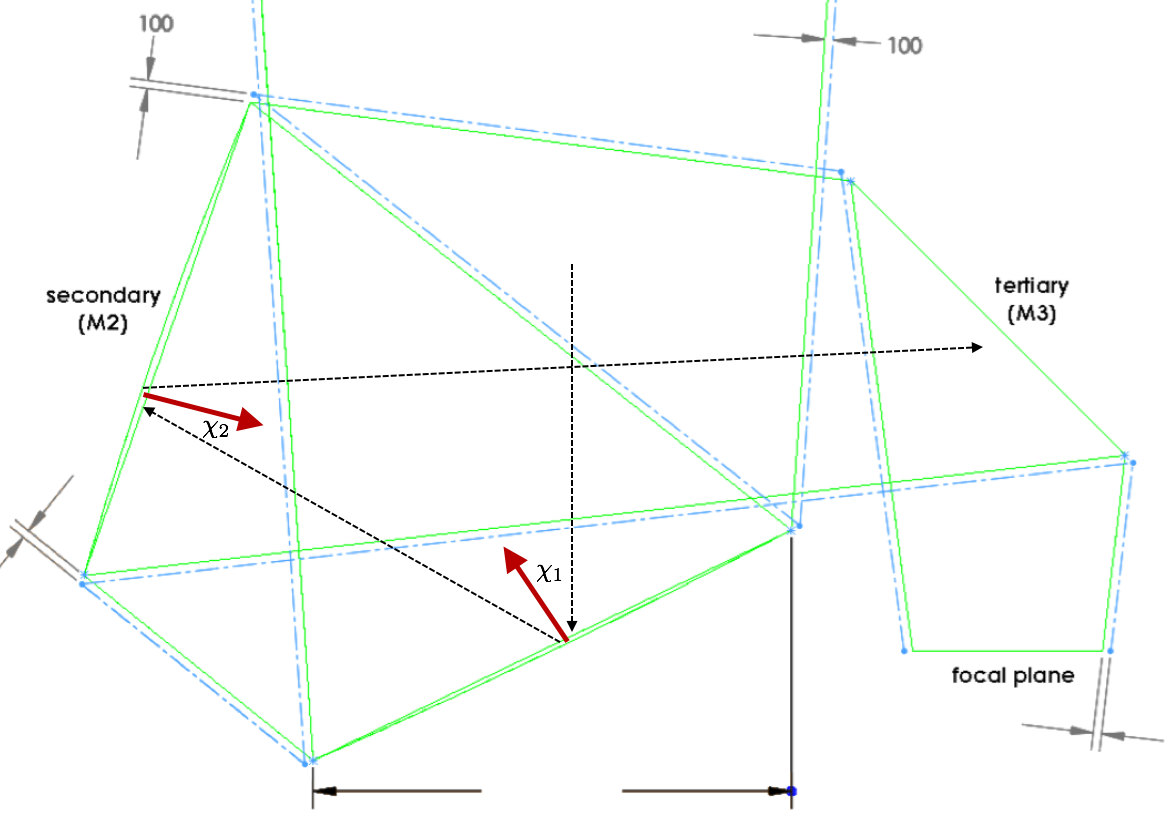
\includegraphics[width=.8\linewidth]{IncidentAngles.png}
  \caption{
  Above is the CCAT optical design, and the angles $\chi_1$ and $\chi_2$ for a given sample trajectory.
  }
  \label{fig:IncidentAngles}
\end{figure}

\subsubsection{Lenses}
\tab The $I\rightarrow P$ coefficients for the lenses was estimated by Brian Koopman for the ACTPol telescope, by propagating unpolarized light throught the system until it reached the detector array using Code V. 
This is data shown in Figure \ref{fig:IP-array}. 
The \ip varies from .12\% on the edge of the array to less than .015\% towards the center.
Because there are three lenses included in the calculation, the individual \ip of each lens is simply the total divided by 3, which gives us .04\% and .005\% for the edge and center respectively.
The total IP for the Large Aperture system can be seen in Table \ref{table:LAT_ip}.
\begin{figure}[t!]
	\centering
  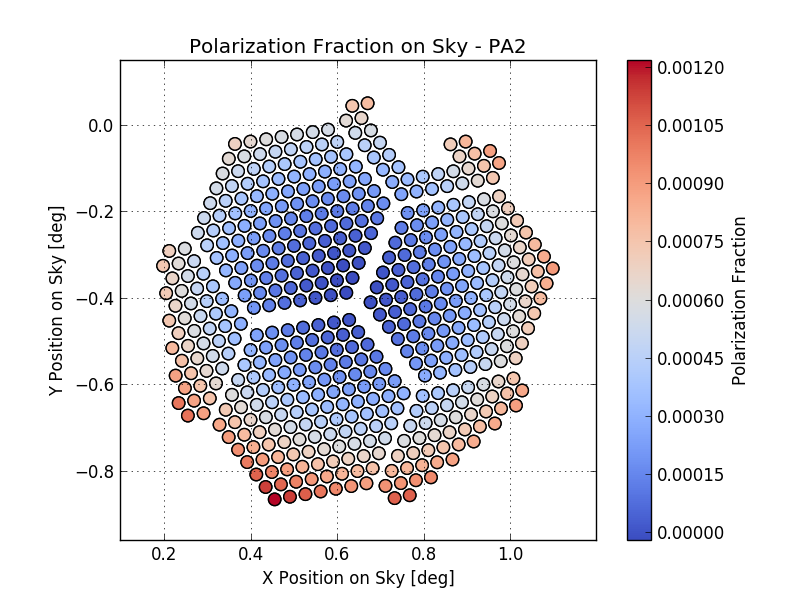
\includegraphics[width=.8\linewidth]{images/pa2_polarization_fraction.png}
  \caption{$I\rightarrow P$ coefficients due to lenses across the detector array of ACTPol.}
  \label{fig:IP-array}
\end{figure}

\subsubsection{Mesh Filters}
\tab Though it is not currently included in the calculation, it may also necessary to consider \ip coming from the mesh filters. 
The $s$ and $p$ transmission of our filters are given in \cite{pisano_polarisation_2006} for incident angles of 
$\chi = 0\degree \t{ and } \chi = 15\degree$ for frequencies above 150 GHz.
From the paper alone, we are able to see that the $s$ and $p$ transmissions are indistinguishable at 0\degree, 
and at 15\degree the maximum \ip in our desired frequency range is about .1\%.

\tab This is more than we actually expect, since the maximum incident angle being considered
around 7.5\degree, and this only occurs at the very edges of the beam.

Additional work is required to come up with a more realistic upper bound on the \ip.

\begin{table}[h]
\centering

\begin{tabular}{|c|c|c|c|c|c|}
\hline
Freq (GHz) & Primary Mirror IP & Secondary Mirror IP & \multicolumn{3}{|c|}{Total $a_4$ (\%)}  \\
\hline
 &&& Pos 1 & Pos 2 & Pos 3 \\
 \hline
27 & 0.011 & 0.006  & 0.018  & 0.058 & 0.098 \\
39 & 0.014 & 0.008  & 0.021  & 0.061 & 0.101 \\
93 & 0.021 & 0.012  & 0.033  & 0.073 & 0.113 \\
145 & 0.026 & 0.015  & 0.041  & 0.081 & 0.121 \\
233 & 0.033 & 0.019  & 0.052  & 0.092 & 0.132 \\
\hline
\end{tabular}
\caption{ Above are the IP coefficients and total $a_4$ for the Large Aperture telescope.
Using a lens IP of 0.04\%, the total $a_4$ is just given the sum of the two mirrors, added to the lens IP times the number of lenses in front of the HWP.
The locations and temperatures of the HWP for each position are given in table \ref{table:SO_OpticalChain}.
}
\label{table:LAT_ip}
\end{table}



\subsection{Small Aperture \ip}

Unlike the large aperture system, rays hitting a given pixel enter the optics parallel to one another. 
Because of this a simple plane wave analysis should be reasonably accurate to calculate the IP of each element. 
This can be done by applying the Fresnel equations at each boundary.
For stacks of thin films, this can easily be done using the transfer matrix method described in \cite{essinger-hileman_transfer_2013} using the python tmm package. 
We calculate the IP coefficient by taking the transmission of s and p-waves separately and calculating the polarized fraction:
\[\text{IP} = \frac{T_p - T_s}{T_p + T_s}.\]
We can then average this over the bandwidth of the detectors.
The major sources of \ip leakage that we consider are the window and the two aluminum filters which are on the sky-side of the HWP.
The IP coefficients and total $a_4$ of the system can be seen in Table \ref{table:SAT_ip}.

The magnitude of the \ip coefficient from this analysis is greatly dependent on the AR coating used. 
The AR coating currently used has two layers on each side, one with index of refraction $n = n_0^{1/3}$ followed by $n = n_0^{2/3}$, and the reverse on the opposite side.
$n_0$ is the index of refraction for the element being coated.
The thickness of each coat is $d = \frac{\lambda_0}{4 n}$ where $\lambda_0$ is the wavelength the coating is optimized for. 
This method of coating works fairly evenly from 93 GHz to 145 GHz, and the current optimized wavelength is $\lambda_0 = 2.5$ mm, or a frequency of 120 GHz.



One issue with the calculation is the presence of Fabry-P\`{e}rot interference between filters.
Because of this the IP coefficient of the two Aluminum filters is dependent on the distance between them, as seen in Figure \ref{fig:IP_vs_distance}.
For the time being we are calculating the IP of each filter in isolation, which is the same as the IP that the filters approach as the distance between them grows to infinity.
This effect may not be real because there are many IR blockers between the Aluminum filter which may change the calculation, 
but if it is real it might need to be considered when choosing the distance between the two filters.
The IP for each filter is again given in Table \ref{table:SAT_ip}.

Another issue on the Small Aperture system is that many of the sources of IP are warm.
The window is at room temperature, and the filters are at $82\degree$ and $42\degree$.
This means polarized emission must be considered for all of the elements rather than just the Mirrors, as was done for the Large Aperture Telescope. 
Though the IP coefficients for the window and filters are fairly small,
the polarized emission increases the $\A4$ signal quite significantly.

\begin{figure}[t!]
	\centering
  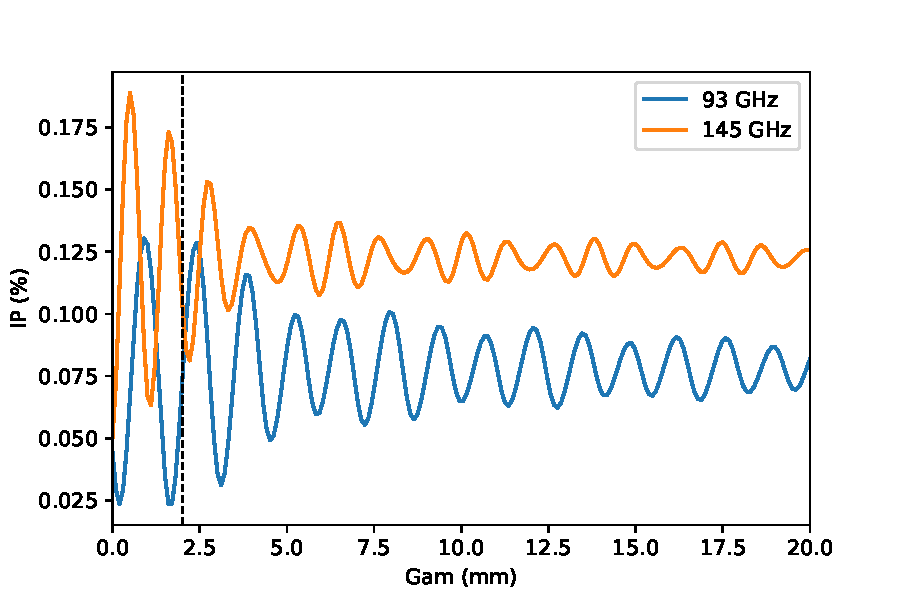
\includegraphics[width=.8\linewidth]{ip_vs_gap_filter_only.pdf}
  \caption{$IP$ coefficient as a function of distance for a system with just two aluminum filters separated by a gap.
  The incident angle is 7.5$\degree$, and frequencies of both 93 and 145 GHz are shown. 
  The black dotted line is at 2 mm, the current distance being considered.
  }
  \label{fig:IP_vs_distance}
\end{figure}



\begin{table}[h]
\centering

\begin{tabular}{|c|c|c|c|c|c|c|}
\hline
$\theta $       & \multicolumn{2}{|c|}{Window IP ($\%$)} & \multicolumn{2}{|c|}{Aluminum Filter IP ($\%$)}  & \multicolumn{2}{|c|}{Total $a_4$ ($\%$)}           \\
\hline
 & 95 GHz & 145 GHz & 95 GHz & 145 GHz & 95 GHz & 145 GHz\\
 \hline
7.5$\degree$ & 0.007 & 0.011 & 0.037 & 0.056 & 0.080 & 0.124\\
10.0$\degree$ & 0.011 & 0.020 & 0.064 & 0.102 & 0.140 & 0.224\\
12.5$\degree$ & 0.016 & 0.032 & 0.098 & 0.164 & 0.213 & 0.360\\
15.0$\degree$ & 0.022 & 0.049 & 0.138 & 0.243 & 0.298 & 0.535\\
\hline
\end{tabular}
\caption{ Above are the band averaged IP coefficients for the window and aluminum filters at 93 and 145 GHz for the Small Aperture Telescope.
 $\theta$ is the incident angle of the lighton the surface.
}
\label{table:SAT_ip}
\end{table}

\section{Propagation}

\tab Using this information the power is propagated through each element.
In this first iteration, if $P_{n}^{u/p}(\nu)$ is the unpolarized / polarized incident power on the $n^\t{th}$ optical element, 
the incident power on the $(n+1)^\t{th}$ element is given by
\begin{align}
P_{n+1}^u(\nu) &= P_n^u(\nu) \eta_n^u(\nu) (1 - \eta_n^{\t{ip}}(\nu)) + A\Omega(\nu) \; \varepsilon_n^u(\nu) B(\nu,T_n)\\
P_{n+1}^p(\nu) &= P_n^u(\nu) \eta_n^u(\nu) \eta_n^{\t{ip}}(\nu) +  P_n^p(\nu) \eta_n^p(\nu) + A\Omega(\nu) \; \varepsilon_n^p(\nu) B(\nu,T_n)
\end{align}
where $\eta_n^{u/p}$ is the unpolarized/polarized efficiency of element $n$, $\eta_n^\t{ip}$ is the \ip coefficient, $\varepsilon_n^{u/p}$
is the unpolarized/polarized emissivity, and $B(\nu,T)$ is the spectral brightness.

\tab The absorption and reflection coefficients for the Large Aperture Telescope are given in the optical chain file and shown in Table 
\ref{table:SO_OpticalChain}. Additional info such as scattering and spillover coefficients are also given.
Because elements are in thermal equilibrium, the absorption is equal to the emissivity $\varepsilon$.
The only exception to this is the primary mirror, where spillover onto heated surfaces adds additional emissivity.
The efficiency $\eta$ is then given by subtracting each coefficient from 1:
\[\eta_n = 1 - \t{abs}_n - \t{refl}_n - \t{scatt}_n\]

\tab After the HWP, additional polarized signal no long contributes to our measurement, 
so the propagation of the polarized power simply becomes
\begin{align}
P_{n+1}^p(\nu) &=  P_n^p(\nu) \eta_n^p(\nu) 
\end{align}

The total unpolarized/polarized power on the detector is then
\[
P^{u} = \frac{1}{2}\int_{\nu_\t{low}}^{\nu_\t{high}} P_\t{det}^u(\nu) d\nu,
\qquad \qquad
P^{p} = \int_{\nu_\t{low}}^{\nu_\t{high}} P_\t{det}^p(\nu) d\nu.
\]
$P_\t{det}$ is the power once the efficiency of the detector is already taken into account. 
$A\Omega$ is already accounted for in the propagation.
The factor of 1/2 is needed when calculating the unpolarized power because we are measuring a single linear polarization,
while it is not included in the polarized power since we do not know the orientation of the polarization of the incoming light, 
and are looking for the maximum value.



\section{$\A4$ Calculation}

\subsection{Large Aperture Results}

\tab Since these calculations are very similar to those done in Charlie Hill's sensitivity code,
our code was built to be compatible with his input files.
The model used is the 45 cm aperture and silicon lenses for various HWP positions:
between the first lense and the window, between the second and first lenses, and between the 2nd lens and the aperture.
The optical chain and HWP positions are shown in Table \ref{table:SO_OpticalChain}.
The HWPSS seen by the detector for each HWP position is shown in Table \ref{table:SO_powers}.
The $a_4$ coefficients for various frequencies and HWP positions are given in Table \ref{table:LAT_ip}.



%
%\begin{table}
%	\centering
%	\begin{tabular}{ |c|c|c|c|c| } 
%		\hline
%		& \multicolumn{2}{|c|}{ $\A4$ (pW)} & \multicolumn{2}{|c|}{ $\A4$ (K$_\t{CMB}$)}\\ 
%		\hline
%		& 93 GHz & 145 GHz & 93 GHz & 145 GHz\\
%		\hline
%		Pos 1 & 0.083  & 0.119 & 0.223 & 0.375 \\
%		Pos 2 & 0.089 & 0.127 & 0.237 & 0.399 \\
%		\hline  
%	\end{tabular}
%	\caption{ Calculated $\AI$ for the optical chain in table \ref{table:SO_OpticalChain} at the three positions shown.
%		These numbers are calculated for a detector at the edge of the array, with a lens IP of 0.04\%.
%		The power is given in pW at the detector, and K$_\text{CMB}$ at the entrance of the telescope.
%	}
%	\label{table:SO_powers}
%\end{table}



\begin{table}
\centering
\begin{tabular}{ |c|c|c|c|c|c|c| } 
  \hline
   & \multicolumn{3}{|c|}{Large Aperture $\A4$ (pW)} & \multicolumn{3}{|c|}{Large Aperture $\A4$ (K$_\t{CMB}$)}\\ 
  \hline
  freq(GHz) & pos 1   & pos 2 & pos 3 & pos 1 & pos 2 & pos 3\\ \hline
 27 &  0.00078 & 0.00083 & 0.00090 & 0.0978 & 0.1037 & 0.1125 \\ 
 39 &  0.00347 & 0.00376 & 0.00414 & 0.1201 & 0.1301 & 0.1431 \\ 
 93 &  0.01055 & 0.01125 & 0.01208 & 0.2231 & 0.2379 & 0.2555 \\ 
145 &  0.02605 & 0.02771 & 0.02957 & 0.3757 & 0.3996 & 0.4264\\ 
233 &  0.08141 & 0.08881 & 0.09650 & 0.9720 & 1.0603 & 1.1520\\ 
  \hline  
\end{tabular}
\caption{ Calculated $\AI$ for the optical chain in table \ref{table:SO_OpticalChain} at the three positions shown.
These numbers are calculated for a detector at the edge of the array, with a lens IP of 0.04\%.
The power is given in pW at the detector, and K$_\text{CMB}$ at the entrance of the telescope.
}
\label{table:SO_powers}
\end{table}


\subsection{Small Aperture Results}

The optical chain used for the small aperture is given in table \ref{table:SO_OpticalChain}. 
The efficiency of the aluminum filters is calculated using the dielectric loss function (taken from Charlie Hill's code):
\[\t{eff} = 1 - \exp\left\{- \frac{2 \pi n \delta d}{\lambda}\right\}\]
where $n$ is the index of refraction, $\delta$ the loss tangent, and $d$ the thickness of the filter.
For these aluminum filters $n = 1.3$, $d = 2\text{ mm}$ and $\delta = .5$. 
I don't quite understand how the units in Charlies code work out, because it requires $\lambda$ to be in nm.

$\A4$ for a detector at the edge of the array for various incident angles are given in Table \ref{table:smallAp_A4}.
For the small aperture telescope, the f-number and FOV have not yet been decided. 
Because the f-number determines the aperture efficiency, changing this changes the polarized power at the detector.
In order to avoid this, the power (pW) that is given is the equivalent power at the start of the telescope.
That is, the total telescope efficiency has been divided out making it independent of f-number.


\begin{table}[h]
\centering

\begin{tabular}{|c|c|c|c|c|}
\hline
$\theta$ & \multicolumn{2}{|c|}{$\A4 $ (pW)}&  \multicolumn{2}{|c|}{$\A4 $ (K$_\text{CMB}$)} \\
\hline
      & 93 GHz   & 145 GHz  & 93 GHz & 145 GHz         \\
\hline
7.5$\degree$ & 0.013 & 0.024 & 0.035 & 0.074 \\
10.0$\degree$ & 0.023 & 0.043 & 0.060 & 0.135 \\
12.5$\degree$ & 0.034 & 0.069 & 0.092 & 0.216 \\
15.0$\degree$ & 0.048 & 0.102 & 0.129 & 0.321 \\
\hline
\end{tabular}
\caption{ $\A4$ for the small aperture telescope for various incident angles. 
When the power is given in pW, it is the equivalent power entering the telescope rather than the power at the detector.
}
\label{table:smallAp_A4}
\end{table}



\subsection{Polarbear}
\tab For a simplified comparison, we used the same optical chain as SO, but with a HWP in between the first and second mirrors.
For the primary mirror we use 32.5\degree, as stated in \cite{takakura_performance_2017}. At $\nu = 145 \t{ GHz}$ this gives a final 
HWPPS of $\AI = .029175 \t{ pW}$. 
Using the conversion $\eta = .18 \t{ pW/K}$, this is 162 mK.
This is consistent with the average measurements given in Table 1 of \cite{takakura_performance_2017}, which is about 160 mK.


\subsection{EBEX}


\tab For our comparison with EBEX the optical chain used is from Christopher Geach's memo on May 1st.
In his analysis Christopher calculates the average polarization fraction across the curved mirror
\[p(\chi) = \frac{\sin^2 \chi}{1 + \cos^2 \chi}\]
to be 15.6\% for the primary mirror and 6.4\% for the secondary mirror. 
This corresponds to the angles $31.3\degree$ and $20.3 \degree$.
At 145 GHz, the \ip of the field lens is about 2.7\% towards the edge of the array.
Using these values we end up with $\AI = .2218 \t{ pW}$, which is larger than their observed value of 0.158 pW.

\tab A possible reason for this is because 2.7\% is the maximum \ip value throughout the detector. 
Decreasing this coefficient to 1.7\% gives us $\AI = .154 \t{ pW}$ which is much closer to the measured result.





\section{$\A2$ Calculation}
\subsection{Calculation}
\tab Using the propagation method described in the sections above, the incident unpolarized power on the HWP plate $P^u_\t{HWP}$ can be calculated. 
The HWP has a Mueller matrix :
\[
M_\t{HWP} = \left(
\begin{array}{cccc}
T & \rho & 0 & 0 \\
\rho & T & 0 & 0 \\
0 & 0 & c & -s\\
0 & 0 & s & c
\end{array}
\right).
\]
The Mueller coefficients $T,\; \rho,\;c,$ and $s$ at each frequency were calculated by Martina for HWPs at each frequency with an anti-reflective coating.
$T$ and $\rho$ determine $\A2$ and are shown in Figure \ref{fig:Mueller_Elements} at a frequency of 150 GHz.

\begin{figure}[t!]
	\centering
  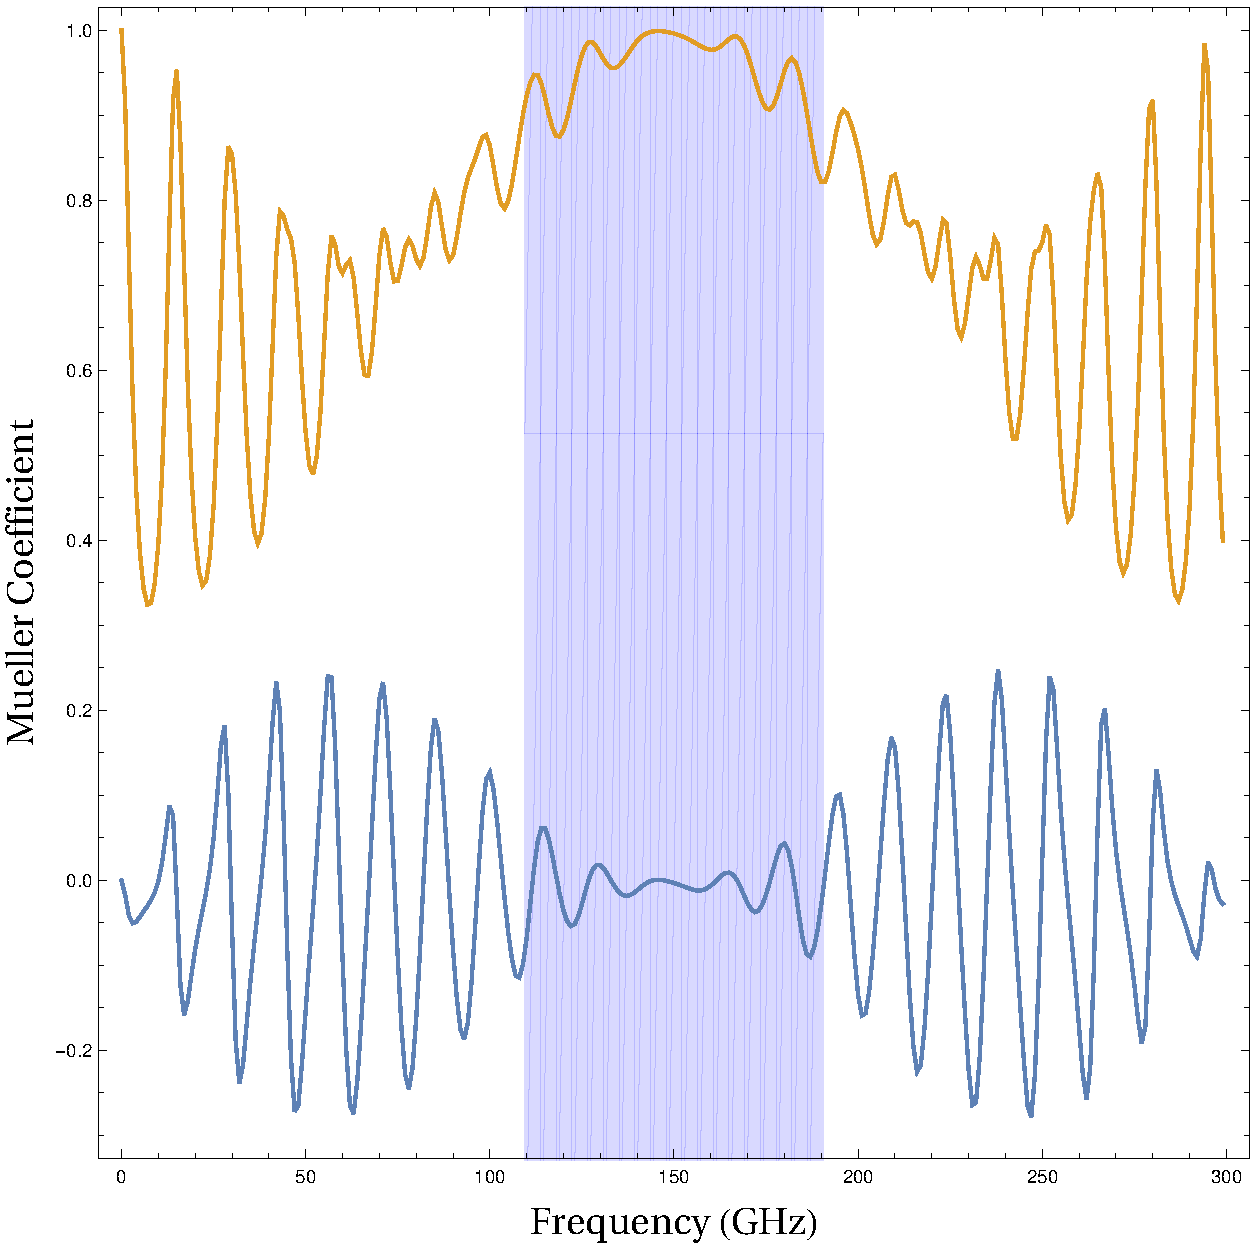
\includegraphics[width=.6\linewidth]{images/Mueller_150GHz.pdf}
  \caption{Shown above are the simulated Mueller elements of the HWP Mueller Matrix at 150GHz with anti-reflective coating. 
  	The orange line is T, the transmission coefficient of I and Q stokes parameters, and the blue line is 
  	$\rho$, the mixing coefficient between I and Q. The blue area is the range of the detector.}
  \label{fig:Mueller_Elements}
\end{figure}

\tab From $M_\t{HWP}$ we can see that the \ip coefficient and thus the polarized emissivity is given by $\rho$. 
$a_2$ is then calculated as the average value of $\rho$ over the detector bandwidth, and values are give in Table \ref{table:SO_a2}.
Since emitted polarized light, and the light that is polarized through \ip are out of phase they are subtracted from one another, and the output polarized power of the HWP is given by
\[
P^p_{\t{HWP} + 1}(\nu)= \rho(\nu) \left(P^u_\t{HWP}(\nu) - A \Omega(\nu) B(\nu, T_\t{HWP}) \right) 	
\]

\tab To calculate $\A2$ we then need $\eta_\t{det}$, the combined efficiency of all elements between the HWP and the detector.
We then integrate over the range of the detector to get
\[
\A2 = \abs{ \int_{\nu_\t{low}}^{\nu_\t{high}} \eta_\t{det}(\nu) P^p_{\t{HWP} + 1} d\nu }.
\]




\subsection{Results}


Result for $a_2$ and $\A2$ can be seen in Table \ref{table:SO_a2}




\begin{table}
\centering
\begin{tabular}{ |c|c|c|c|} 
	\hline
	freq (GHz) &  $a_2\; (\%)$ & $\A2$ (pW)  & $\A2$ ($K_\t{CMB}$) \\ \hline
	27.0  & 0.8963 & 0.0017 & 0.212 \\ 
	39.0  & 0.4152 & 0.004  & 0.1391\\ 
	93.0  & 0.3167 & 0.0067 & 0.1413\\ 
	145.0 & 0.3576 & 0.0165 & 0.2389\\ 
	233.0 & 0.6395 & 0.1211 & 1.446 \\ 
	\hline	
\end{tabular}



\caption{ $a_2$ and $\A2$ for the optical system given in table \ref{table:SO_OpticalChain} with the HWP at 4 K. 
Only one position is shown because changing the position of the HWP only alters the result by about .01 fW. 
}
\label{table:SO_a2}
\end{table}



\subsection{Small Aperture}
The Small Aperture calculation of $\A2$ and $a_2$ is identical to that of the large aperture calculation,
and the same HWP calculations are used. 
As we did for $\A4$, the power given in pW is the equivalent power entering the telescope rather than at the detector. 

The results can be seen in Table \ref{table:smallAp_A2}.
$\A2$ is mainly controlled by the HWP Mueller matrix, which doesn't change much as a function of incident angle as seen in figure \ref{fig:Mueller_incAngles}.
Based on this, the little change seen in $\A2$ makes sense.

 \begin{table}[h]
\centering

\begin{tabular}{|c|c|c|c|c|}
\hline
$\theta$ & \multicolumn{2}{|c|}{$\A2 $ (pW)}&  \multicolumn{2}{|c|}{$\A2 $ (K$_\text{CMB}$)} \\
\hline
      & 90 GHz   & 150 GHz  & 90 GHz & 150 GHz         \\
\hline
8$\degree$   & 0.0499 & 0.0752 & 0.133  & 0.236\\
10$\degree$  & 0.0482 & 0.0764 & 0.129  & 0.244\\
15$\degree$  & 0.042  & 0.0866 & 0.118  & 0.272\\\hline
\end{tabular}
\caption{ $\A2$ for the small aperture telescope for various incident angles. 
When the power is given in pW, it is the equivalent power entering the telescope rather than the power at the detector.
}
\label{table:smallAp_A2}
\end{table}


\begin{figure}[t!]
	\centering
  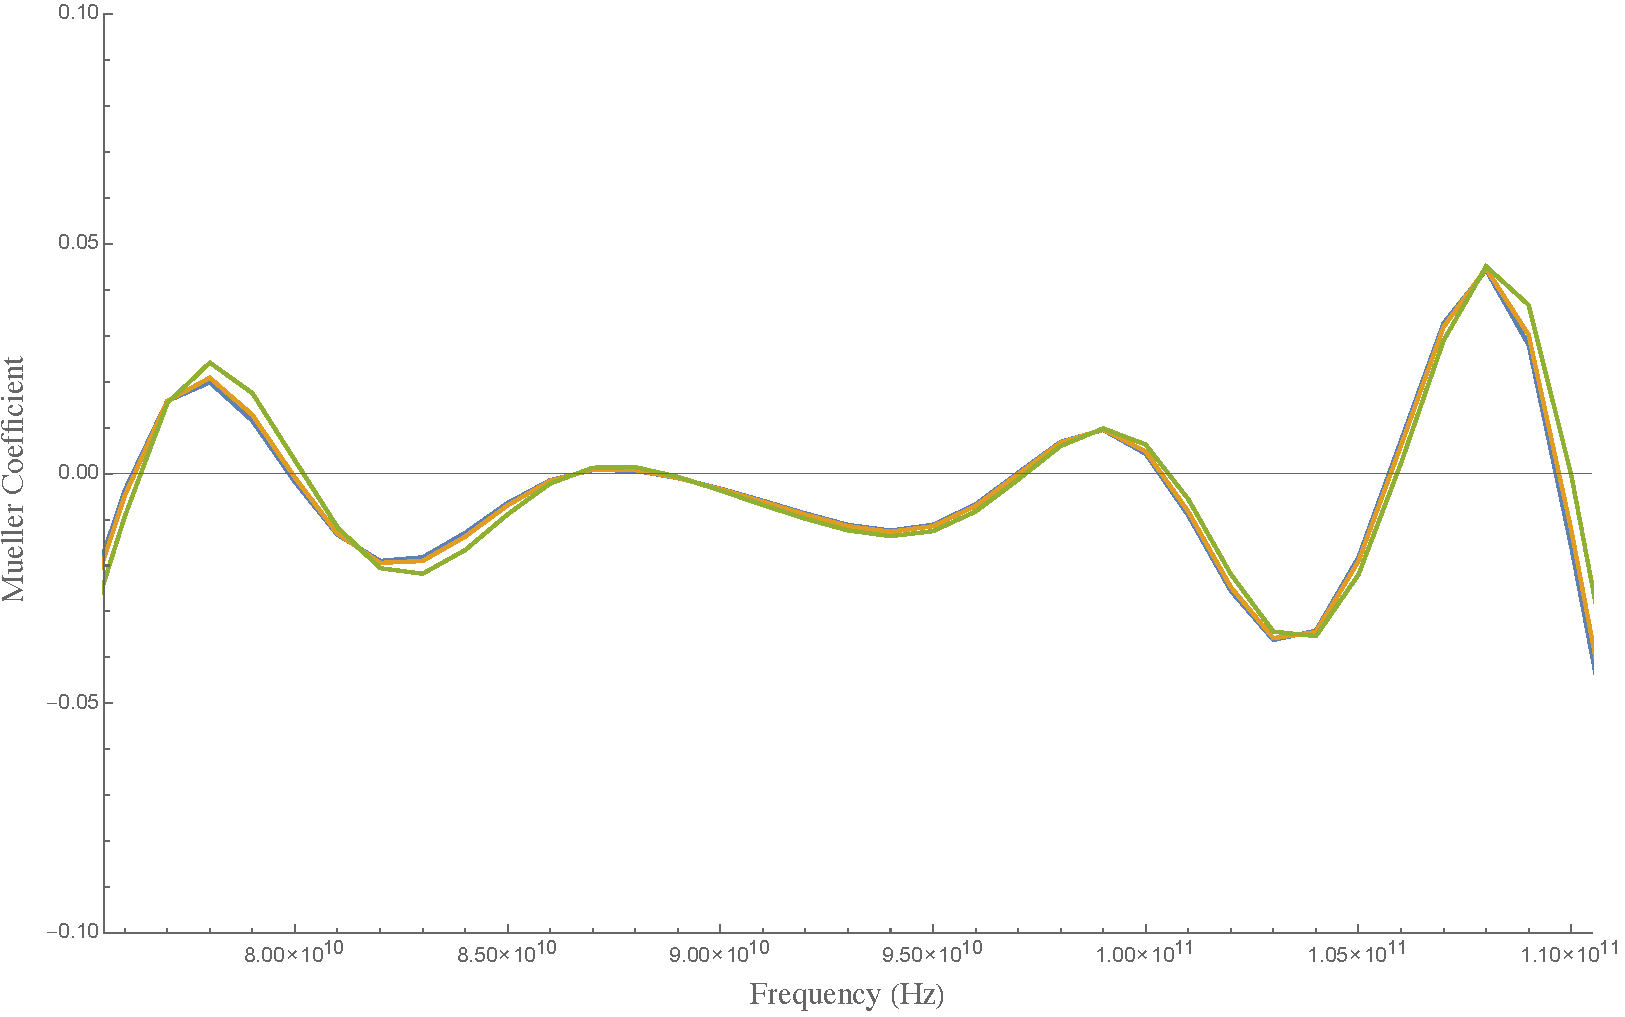
\includegraphics[width=.6\linewidth]{MuellerIncAngles.pdf}
  \caption{Shown above is the $\rho$ Mueller coefficient for incident angles of $8\degree$ (blue), $10\degree$ (orange), and $15\degree$ (green) for a band centered at 90 GHz}
  \label{fig:Mueller_incAngles}
\end{figure}

\section*{}




\begin{table}

\centering
\begin{tabular}{ |l|c|c|} 
	\hline
	\multicolumn{3}{|c|}{SO Large Aperture [145 GHz, 233 GHz]}\\
	\hline
	 Name 		& Temp (K)	& Abs 		\\ \hline
	 Mirror 	&	273		& [0.002, 0.005] 	\\
	 \hline \multicolumn{3}{|c|}{POLARBEAR HWP }	\\ \hline
	 Mirror 	&	273		& [0.002, 0.005]	\\
	 Window 	&	265		& [0.005, 0.010] 	 \\
	 \hline \multicolumn{3}{|c|}{HWP pos 1 (80 K)}	\\ \hline
	 IRShaders 	&	80		& [0.001, 0.001]	\\
	 IRShaders 	&	40		& [0.001, 0.001]	\\
	 LowPass 	&	10		& [0.010, 0.010] 	\\
	 Lens 		&	4.5		& [0.007, 0.011] 	 \\
	 \hline \multicolumn{3}{|c|}{HWP pos 2 (4 K)}	\\ \hline
	 Lens 		&	1.2		& [0.007, 0.011] 	 \\
	 \hline \multicolumn{3}{|c|}{HWP pos 3 (4 K?)}	\\ \hline
	 Aperture 	&	1.2		&  NA  			 	\\
	 Lens 		&	1.2		& [0.007, 0.011] 	 \\
	 LowPass 	&	1.2		& [0.010, 0.010] 	 \\
	 LowPass 	&	1.2		& [0.010, 0.010] 	 \\
	 LowPass 	&	.1		& [0.010, 0.010] 	 \\
	\hline	
\end{tabular}
\!
\begin{tabular}{|c|c|c|}
\hline
\multicolumn{3}{|c|}{SO Small Aperture [93 GHz, 145 GHz]}\\
\hline
Name & Temp & Abs \\
\hline
Window + ARC		& 300.0  & [0.005,0.010]	\\
IRShader1	& 298.0  & [0.001,0.001]	\\
IRShader2	& 293.0  & [0.001,0.001]	\\
IRShader3	& 290.0  & [0.001,0.001]	\\
IRShader4	& 276.0  & [0.001,0.001]	\\
AluminaF + ARC	& 82.00  &  NA			  	\\
IRShader1	& 76.00  & [0.001,0.001]	\\
IRShader2	& 70.00  & [0.001,0.001]	\\
IRShader3	& 65.00  & [0.001,0.001]	\\
IRShader4	& 61.00  & [0.001,0.001]	\\
AluminaF + ARC	& 42.00  &  NA			  	\\
\hline
\multicolumn{3}{|c|}{HWP} \\
\hline
AluminaF	& 40.00  &  NA			  	\\
AluminaF	& 5.000  &  NA			  	\\
LowPass1	& 4.000  & [0.010,0.010]	\\
Aperture	& 1.000  & NA	       	\\
Lens		& 1.000  &  NA			  	\\
Lens		& 1.000  &  NA			  	\\
LowPass1	& 0.100  & [0.010,0.010]	\\

\hline
\end{tabular}

\caption{Our current optical chain with a 45 cm aperture and silicon lenses.
Shown is also the three HWP positions which we have considered, and the HWP position used for our POLARBEAR comparison.
}

\label{table:SO_OpticalChain}
\end{table}






% \begin{table}
% \centering
% \begin{tabular}{ |c|c|c|c| } 
%   \hline
%    & \multicolumn{3}{|c|}{Large Aperture $\A4$ (pW)}\\
%   \hline
%   freq(GHz) & pos 1   & pos 2 & pos 3 \\ \hline
%  27 &  \text{0.00078, 0.00078} &  \text{0.00083, 0.00079} &  \text{0.0009, 0.0008  }  \\ 
%  39 &  \text{0.00347, 0.00347} &  \text{0.00376, 0.00351} &  \text{0.00414, 0.00356}  \\ 
%  93 &  \text{0.01055, 0.01055} &  \text{0.01125, 0.01064} &  \text{0.01208, 0.01074}  \\ 
% 145 &  \text{0.02605, 0.02605} &  \text{0.02771, 0.02626} &  \text{0.02957, 0.02649}  \\ 
% 233 &  \text{0.08141, 0.08141} &  \text{0.08881, 0.08234} &  \text{0.0965, 0.0833  }  \\ 
%   \hline  
% \end{tabular}
% \begin{tabular}{ |c|c|c|c| } 
%   \hline
%    & \multicolumn{3}{|c|}{Large Aperture $\A4$ (K$_\t{CMB}$)}\\
%   \hline
%   freq (GHz) & pos 1  & pos 2 & pos 3 \\ \hline
%    27&  \text{0.0978, 0.0978} & \text{ 0.1037, 0.0985 }& \text{ 0.1125, 0.0996 } \\ 
%    39&  \text{0.1201, 0.1201} & \text{ 0.1301, 0.1214 }& \text{ 0.1431, 0.123  } \\ 
%    93&  \text{0.2231, 0.2231} & \text{ 0.2379, 0.225  }& \text{ 0.2555, 0.2272 } \\ 
%   145&  \text{0.3757, 0.3757} & \text{ 0.3996, 0.3787 }& \text{ 0.4264, 0.382  } \\ 
%   233&  \text{0.972, 0.972  } & \text{ 1.0603, 0.983  }& \text{ 1.152, 0.9945  } \\ 

%   \hline  
% \end{tabular}
% \caption{ Calculated $\AI$ for the optical chain in table \ref{table:SO_OpticalChain} at the three positions shown.
% In each cell, the first number is $\AI$ for a detector towards the edge of the array, and the second number 
% is for a detector towards the center. We present the power in both pW and K$_\t{CMB}$
% }
% \label{table:SO_powers}
% \end{table}












\printbibliography


\end{document}

